% Pipeline Visualizations for CFAR-STFT Radar Detection
% Compilare: pdflatex pipeline_diagrams.tex
% Necesita: tikz, pgfplots

\documentclass[11pt,a4paper]{article}
\usepackage[utf8]{inputenc}
\usepackage[romanian]{babel}
\usepackage{tikz}
\usepackage{pgfplots}
\usepackage{amsmath,amssymb}
\usepackage{geometry}
\usepackage{xcolor}
\usepackage{float}

\geometry{margin=2cm}
\pgfplotsset{compat=1.18}

\usetikzlibrary{shapes.geometric, arrows.meta, positioning, calc, patterns, decorations.pathreplacing, matrix, fit, backgrounds}

% Culori personalizate
\definecolor{stftblue}{RGB}{66, 133, 244}
\definecolor{cfarorange}{RGB}{255, 152, 0}
\definecolor{dbscangreen}{RGB}{76, 175, 80}
\definecolor{maskpurple}{RGB}{156, 39, 176}
\definecolor{istftred}{RGB}{244, 67, 54}
\definecolor{signalgray}{RGB}{96, 96, 96}

\title{\textbf{Diagrame Pipeline CFAR-STFT}\\[0.5em]
\large Detecția semnalelor radar în sea clutter}
\author{Ingrid Corobana \and Teodora-Ioana Nae}
\date{Ianuarie 2026}

\begin{document}
\maketitle

%% =============================================================================
%% DIAGRAMA 1: Pipeline-ul principal
%% =============================================================================
\section{Pipeline-ul Algoritmului CFAR-STFT}

\begin{figure}[H]
\centering
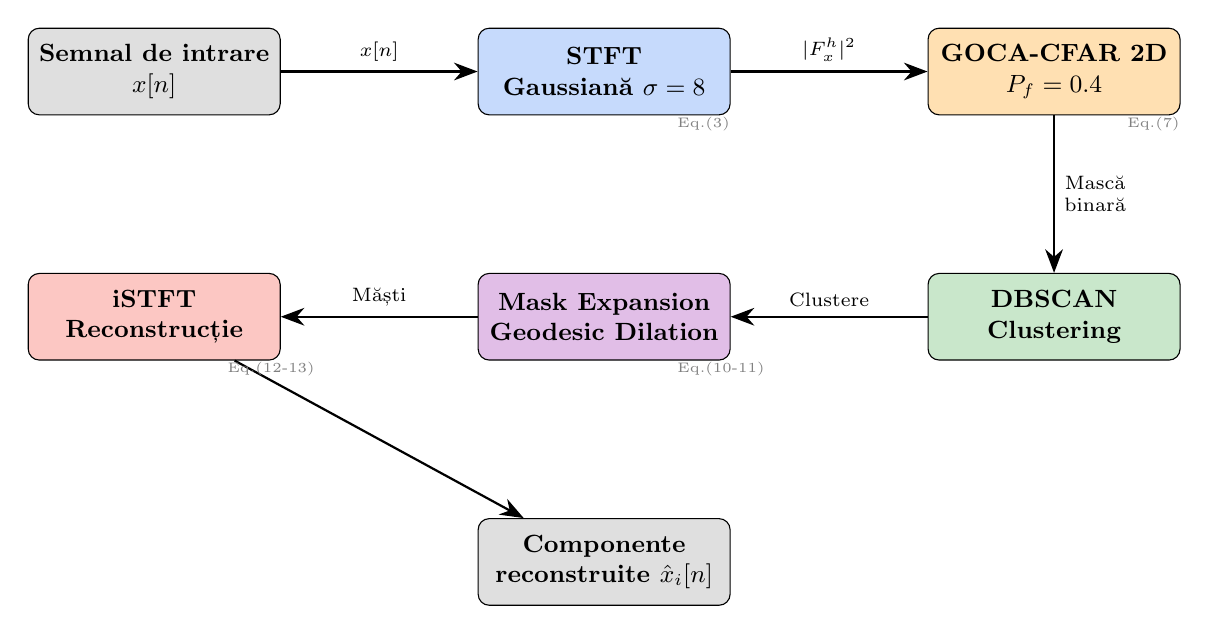
\begin{tikzpicture}[
    node distance=2.2cm and 2.5cm,
    box/.style={rectangle, draw, rounded corners, minimum width=3.2cm, minimum height=1.1cm, align=center, font=\small\bfseries},
    arrow/.style={-{Stealth[length=3mm]}, thick},
    label/.style={font=\scriptsize, align=center},
    eqlabel/.style={font=\tiny, text=gray}
]

% Rândul 1: Input -> STFT -> CFAR
\node[box, fill=signalgray!20] (input) {Semnal de intrare\\$x[n]$};

\node[box, fill=stftblue!30, right=of input] (stft) {STFT\\Gaussiană $\sigma=8$};

\node[box, fill=cfarorange!30, right=of stft] (cfar) {GOCA-CFAR 2D\\$P_f=0.4$};

% Rândul 2: DBSCAN -> Mask -> iSTFT
\node[box, fill=dbscangreen!30, below=2cm of cfar] (dbscan) {DBSCAN\\Clustering};

\node[box, fill=maskpurple!30, below=2cm of stft] (mask) {Mask Expansion\\Geodesic Dilation};

\node[box, fill=istftred!30, below=2cm of input] (istft) {iSTFT\\Reconstrucție};

% Rândul 3: Output
\node[box, fill=signalgray!20, below=2cm of mask] (output) {Componente\\reconstruite $\hat{x}_i[n]$};

% Săgeți rândul 1
\draw[arrow] (input) -- node[above, label] {$x[n]$} (stft);
\draw[arrow] (stft) -- node[above, label] {$|F_x^h|^2$} (cfar);

% Săgeți verticale și rândul 2
\draw[arrow] (cfar) -- node[right, label] {Mască\\binară} (dbscan);
\draw[arrow] (dbscan) -- node[above, label] {Clustere} (mask);
\draw[arrow] (mask) -- node[above, label] {Măști} (istft);

% Săgeată finală
\draw[arrow] (istft) -- (output);

% Ecuații (în colțul drept-jos al fiecărui nod)
\node[eqlabel, below right=-0.1cm and -0.8cm of stft] {Eq.(3)};
\node[eqlabel, below right=-0.1cm and -0.8cm of cfar] {Eq.(7)};
\node[eqlabel, below right=-0.1cm and -0.8cm of mask] {Eq.(10-11)};
\node[eqlabel, below right=-0.1cm and -0.8cm of istft] {Eq.(12-13)};

\end{tikzpicture}
\caption{Pipeline-ul complet al algoritmului CFAR-STFT pentru extracția componentelor din planul timp-frecvență (conform Abratkiewicz 2022).}
\label{fig:pipeline}
\end{figure}

%% =============================================================================
%% DIAGRAMA 2: Structura celulelor CFAR
%% =============================================================================
\section{Structura Detectorului GOCA-CFAR 2D}

\begin{figure}[H]
\centering
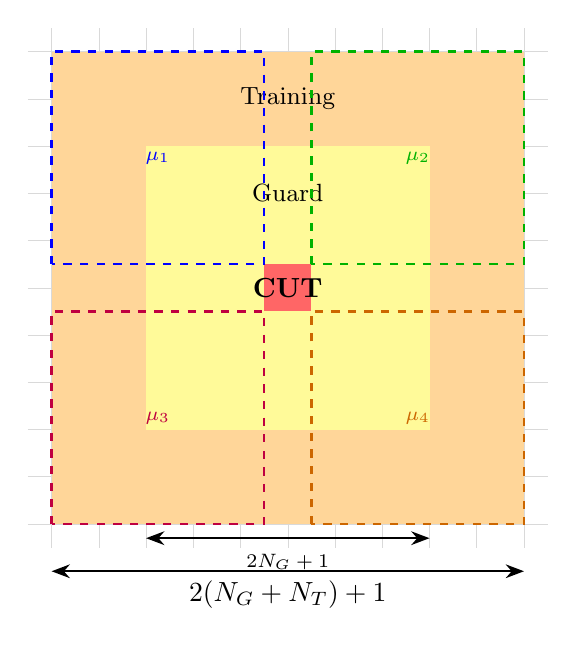
\begin{tikzpicture}[scale=0.6]
    % Grid background
    \draw[step=1, gray!30, very thin] (-5.5,-5.5) grid (5.5,5.5);
    
    % Training cells (outer ring)
    \fill[cfarorange!40] (-5,-5) rectangle (5,5);
    
    % Guard cells (middle ring)
    \fill[yellow!40] (-3,-3) rectangle (3,3);
    
    % CUT (center)
    \fill[red!60] (-0.5,-0.5) rectangle (0.5,0.5);
    
    % Labels pentru regiuni
    \node at (0,0) {\textbf{CUT}};
    \node at (0,2) {\small Guard};
    \node at (0,4) {\small Training};
    
    % Dimensiuni
    \draw[{Stealth}-{Stealth}, thick] (-5,-6) -- (5,-6);
    \node at (0,-6.5) {$2(N_G + N_T) + 1$};
    
    \draw[{Stealth}-{Stealth}, thick] (-3,-5.3) -- (3,-5.3);
    \node at (0,-5.8) {\scriptsize $2N_G + 1$};
    
    % GOCA regions
    \draw[thick, blue, dashed] (-5,0.5) rectangle (-0.5,5);
    \draw[thick, green!70!black, dashed] (0.5,0.5) rectangle (5,5);
    \draw[thick, purple, dashed] (-5,-5) rectangle (-0.5,-0.5);
    \draw[thick, orange!80!black, dashed] (0.5,-5) rectangle (5,-0.5);
    
    \node[blue, font=\scriptsize] at (-2.75,2.75) {$\mu_1$};
    \node[green!70!black, font=\scriptsize] at (2.75,2.75) {$\mu_2$};
    \node[purple, font=\scriptsize] at (-2.75,-2.75) {$\mu_3$};
    \node[orange!80!black, font=\scriptsize] at (2.75,-2.75) {$\mu_4$};
    
\end{tikzpicture}
\hspace{1cm}
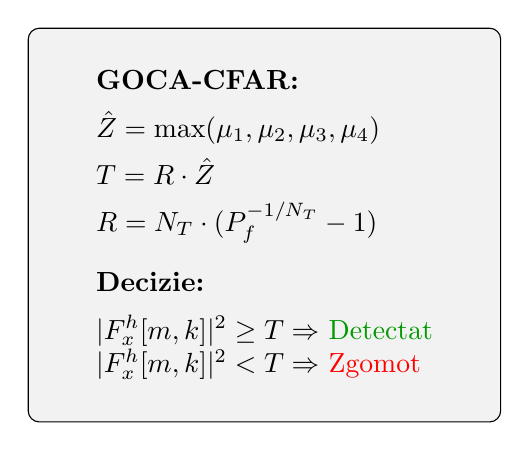
\begin{tikzpicture}[scale=0.9]
    % Formula box
    \node[draw, rounded corners, fill=gray!10, minimum width=6cm, minimum height=5cm, align=left] (formulas) {
        \textbf{GOCA-CFAR:}\\[0.5em]
        $\hat{Z} = \max(\mu_1, \mu_2, \mu_3, \mu_4)$\\[0.5em]
        $T = R \cdot \hat{Z}$\\[0.5em]
        $R = N_T \cdot (P_f^{-1/N_T} - 1)$\\[1em]
        \textbf{Decizie:}\\[0.5em]
        $|F_x^h[m,k]|^2 \geq T \Rightarrow$ \textcolor{green!60!black}{Detectat}\\
        $|F_x^h[m,k]|^2 < T \Rightarrow$ \textcolor{red}{Zgomot}
    };
\end{tikzpicture}
\caption{Structura celulelor GOCA-CFAR 2D. CUT = Cell Under Test (roșu), Guard cells (galben), Training cells (portocaliu). GOCA calculează media în 4 sub-regiuni și ia maximul.}
\label{fig:cfar}
\end{figure}

%% =============================================================================
%% DIAGRAMA 3: Fluxul de date pentru experiment
%% =============================================================================
\section{Configurația Experimentală}

\begin{figure}[H]
\centering
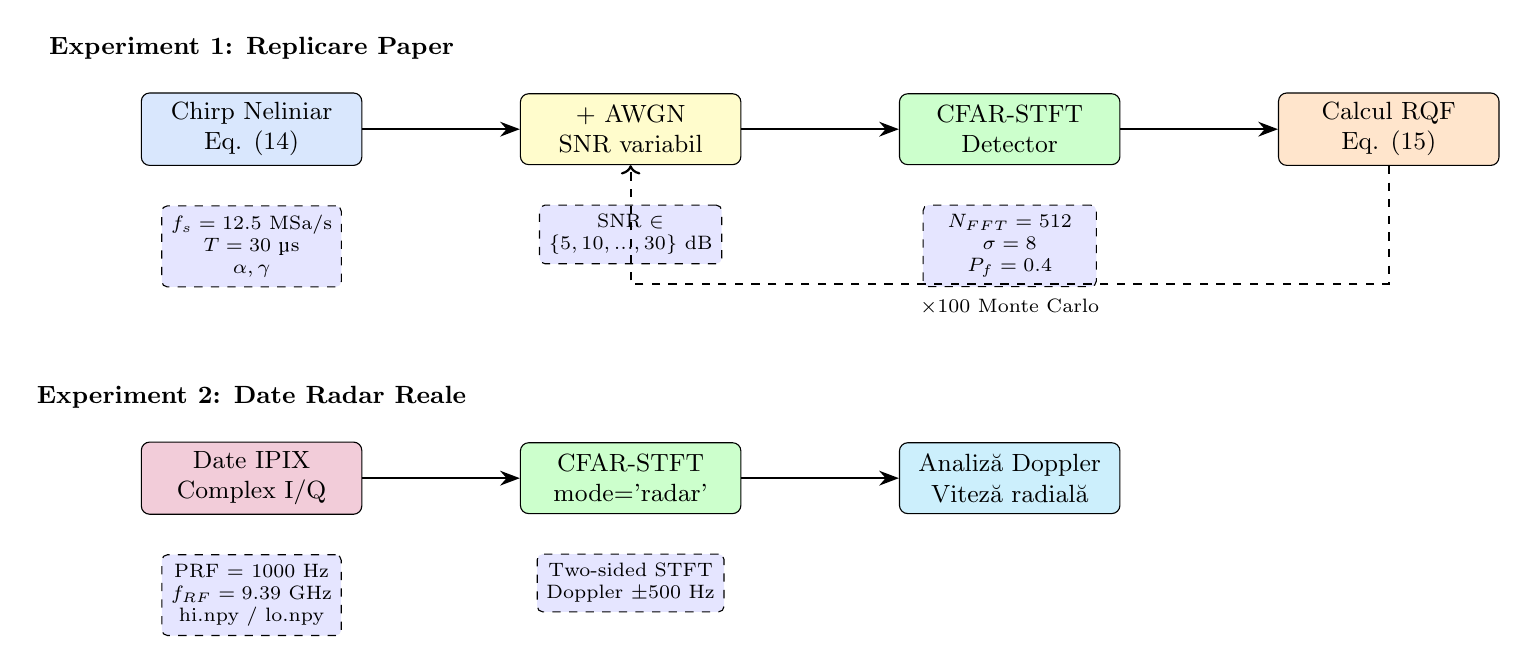
\begin{tikzpicture}[
    node distance=1.2cm and 2cm,
    box/.style={rectangle, draw, rounded corners=3pt, minimum width=2.8cm, minimum height=0.9cm, align=center, font=\small},
    param/.style={rectangle, draw, dashed, rounded corners=2pt, fill=blue!10, minimum width=2.2cm, font=\scriptsize, align=center},
    arrow/.style={-{Stealth[length=2.5mm]}, thick}
]

% Experiment sintetic
\node[box, fill=stftblue!20] (chirp) {Chirp Neliniar\\Eq. (14)};
\node[param, below=0.5cm of chirp] (chirp_params) {$f_s = 12.5$ MSa/s\\$T = 30$ µs\\$\alpha, \gamma$};

\node[box, fill=yellow!20, right=of chirp] (noise) {+ AWGN\\SNR variabil};
\node[param, below=0.5cm of noise] (noise_params) {SNR $\in$\\$\{5,10,...,30\}$ dB};

\node[box, fill=green!20, right=of noise] (detector) {CFAR-STFT\\Detector};
\node[param, below=0.5cm of detector] (det_params) {$N_{FFT}=512$\\$\sigma=8$\\$P_f=0.4$};

\node[box, fill=orange!20, right=of detector] (rqf) {Calcul RQF\\Eq. (15)};

% Săgeți
\draw[arrow] (chirp) -- (noise);
\draw[arrow] (noise) -- (detector);
\draw[arrow] (detector) -- (rqf);

% Monte Carlo loop
\draw[thick, dashed, ->] (rqf.south) -- ++(0,-1.5) -| (noise.south);
\node[font=\scriptsize] at ($(rqf.south)!0.5!(noise.south) + (0,-1.8)$) {$\times 100$ Monte Carlo};

% IPIX experiment (below)
\node[box, fill=purple!20, below=3.5cm of chirp] (ipix) {Date IPIX\\Complex I/Q};
\node[param, below=0.5cm of ipix] (ipix_params) {PRF = 1000 Hz\\$f_{RF} = 9.39$ GHz\\hi.npy / lo.npy};

\node[box, fill=green!20, right=of ipix] (detector2) {CFAR-STFT\\mode='radar'};
\node[param, below=0.5cm of detector2] (det2_params) {Two-sided STFT\\Doppler $\pm 500$ Hz};

\node[box, fill=cyan!20, right=of detector2] (doppler) {Analiză Doppler\\Viteză radială};

\draw[arrow] (ipix) -- (detector2);
\draw[arrow] (detector2) -- (doppler);

% Labels
\node[font=\small\bfseries, above=0.3cm of chirp] {Experiment 1: Replicare Paper};
\node[font=\small\bfseries, above=0.3cm of ipix] {Experiment 2: Date Radar Reale};

\end{tikzpicture}
\caption{Configurația celor două experimente: (sus) replicarea Fig. 6 din paper cu chirp sintetic, (jos) validare pe date IPIX sea clutter.}
\label{fig:experiments}
\end{figure}

%% =============================================================================
%% DIAGRAMA 4: Planul timp-frecvență și procesarea
%% =============================================================================
\section{Procesarea în Planul Timp-Frecvență}

\begin{figure}[H]
\centering
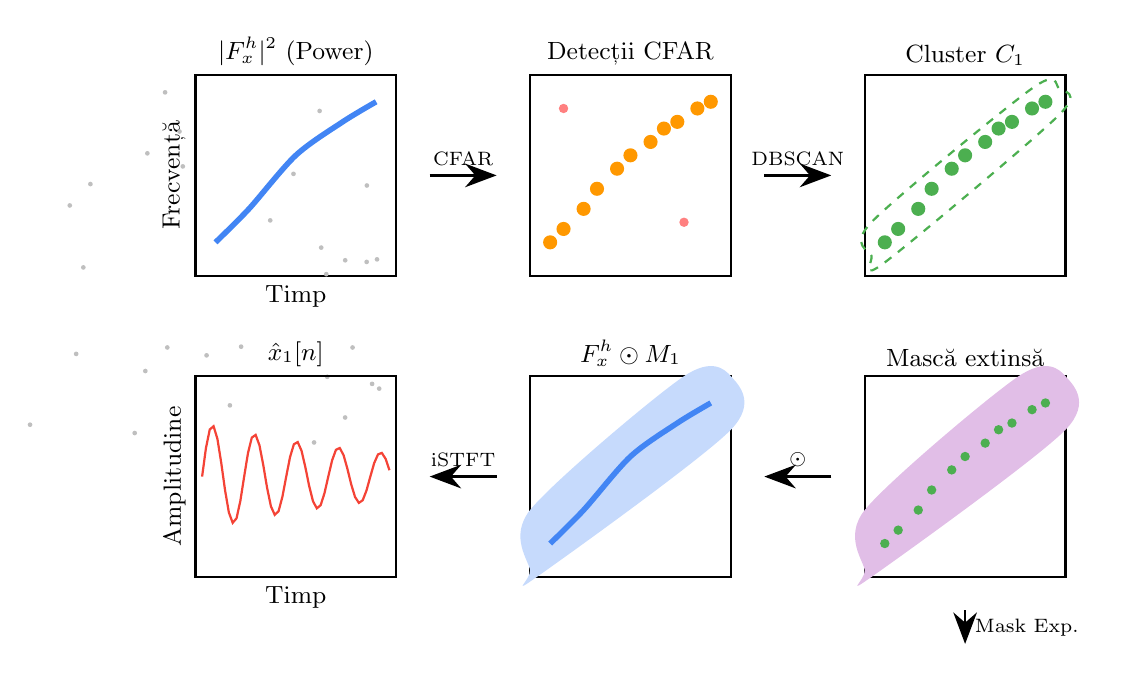
\begin{tikzpicture}[scale=0.85]

% Spectrogram box 1 - Input
\begin{scope}[xshift=0cm]
    \draw[thick] (0,0) rectangle (3,3);
    \node[above] at (1.5,3) {\small $|F_x^h|^2$ (Power)};
    \node[below] at (1.5,0) {\small Timp};
    \node[rotate=90, above] at (0,1.5) {\small Frecvență};
    
    % Signal ridge (curve)
    \draw[thick, stftblue, line width=2pt] plot[smooth] coordinates {(0.3,0.5) (0.8,1.0) (1.5,1.8) (2.2,2.3) (2.7,2.6)};
    
    % Noise dots
    \foreach \i in {1,...,30} {
        \fill[gray!50] (rand*2.8+0.1, rand*2.8+0.1) circle (1pt);
    }
\end{scope}

% Arrow
\draw[-{Stealth[length=4mm]}, thick] (3.5,1.5) -- (4.5,1.5);
\node[above] at (4,1.5) {\scriptsize CFAR};

% Spectrogram box 2 - After CFAR
\begin{scope}[xshift=5cm]
    \draw[thick] (0,0) rectangle (3,3);
    \node[above] at (1.5,3) {\small Detecții CFAR};
    
    % Detected points (on ridge)
    \foreach \x/\y in {0.3/0.5, 0.5/0.7, 0.8/1.0, 1.0/1.3, 1.3/1.6, 1.5/1.8, 1.8/2.0, 2.0/2.2, 2.2/2.3, 2.5/2.5, 2.7/2.6} {
        \fill[cfarorange] (\x, \y) circle (3pt);
    }
    % Some false alarms
    \fill[red!50] (0.5, 2.5) circle (2pt);
    \fill[red!50] (2.3, 0.8) circle (2pt);
\end{scope}

% Arrow
\draw[-{Stealth[length=4mm]}, thick] (8.5,1.5) -- (9.5,1.5);
\node[above] at (9,1.5) {\scriptsize DBSCAN};

% Spectrogram box 3 - After clustering
\begin{scope}[xshift=10cm]
    \draw[thick] (0,0) rectangle (3,3);
    \node[above] at (1.5,3) {\small Cluster $C_1$};
    
    % Clustered points (only the ridge)
    \foreach \x/\y in {0.3/0.5, 0.5/0.7, 0.8/1.0, 1.0/1.3, 1.3/1.6, 1.5/1.8, 1.8/2.0, 2.0/2.2, 2.2/2.3, 2.5/2.5, 2.7/2.6} {
        \fill[dbscangreen] (\x, \y) circle (3pt);
    }
    % Convex hull around cluster
    \draw[dbscangreen, thick, dashed] plot[smooth cycle] coordinates {(0.1,0.3) (0.3,0.2) (2.9,2.4) (2.9,2.8) (2.5,2.8) (0.1,0.8)};
\end{scope}

% Second row
\begin{scope}[yshift=-4.5cm]

% Arrow down from box 3
\draw[-{Stealth[length=4mm]}, thick] (11.5,-0.5) -- (11.5,-1);
\node[right] at (11.5,-0.75) {\scriptsize Mask Exp.};

% Spectrogram box 4 - Expanded mask
\begin{scope}[xshift=10cm]
    \draw[thick] (0,0) rectangle (3,3);
    \node[above] at (1.5,3) {\small Mască extinsă};
    
    % Expanded mask region
    \fill[maskpurple!30] plot[smooth cycle] coordinates {(0.0,0.1) (0.1,0.0) (3.0,2.2) (3.0,3.0) (2.3,3.0) (0.0,1.0)};
    
    % Original points
    \foreach \x/\y in {0.3/0.5, 0.5/0.7, 0.8/1.0, 1.0/1.3, 1.3/1.6, 1.5/1.8, 1.8/2.0, 2.0/2.2, 2.2/2.3, 2.5/2.5, 2.7/2.6} {
        \fill[dbscangreen] (\x, \y) circle (2pt);
    }
\end{scope}

% Arrow
\draw[-{Stealth[length=4mm]}, thick] (9.5,1.5) -- (8.5,1.5);
\node[above] at (9,1.5) {\scriptsize $\odot$};

% Spectrogram box 5 - Masked STFT
\begin{scope}[xshift=5cm]
    \draw[thick] (0,0) rectangle (3,3);
    \node[above] at (1.5,3) {\small $F_x^h \odot M_1$};
    
    % Only the signal part
    \fill[stftblue!30] plot[smooth cycle] coordinates {(0.0,0.1) (0.1,0.0) (3.0,2.2) (3.0,3.0) (2.3,3.0) (0.0,1.0)};
    \draw[thick, stftblue, line width=2pt] plot[smooth] coordinates {(0.3,0.5) (0.8,1.0) (1.5,1.8) (2.2,2.3) (2.7,2.6)};
\end{scope}

% Arrow
\draw[-{Stealth[length=4mm]}, thick] (4.5,1.5) -- (3.5,1.5);
\node[above] at (4,1.5) {\scriptsize iSTFT};

% Output signal
\begin{scope}[xshift=0cm]
    \draw[thick] (0,0) rectangle (3,3);
    \node[above] at (1.5,3) {\small $\hat{x}_1[n]$};
    
    % Reconstructed signal waveform
    \draw[thick, istftred] plot[domain=0:2.8, samples=50] (\x+0.1, {1.5 + 0.8*sin(10*\x r)*exp(-0.3*\x)});
    
    \node[below] at (1.5,0) {\small Timp};
    \node[rotate=90, above] at (0,1.5) {\small Amplitudine};
\end{scope}

\end{scope}

\end{tikzpicture}
\caption{Fluxul de procesare în planul timp-frecvență: spectrograma de putere $\rightarrow$ detecții CFAR $\rightarrow$ clustering DBSCAN $\rightarrow$ extindere mască $\rightarrow$ mascare STFT $\rightarrow$ reconstrucție iSTFT.}
\label{fig:tf_processing}
\end{figure}

%% =============================================================================
%% DIAGRAMA 5: Conversia Doppler-Viteză
%% =============================================================================
\section{Interpretarea Doppler pentru Radar}

\begin{figure}[H]
\centering
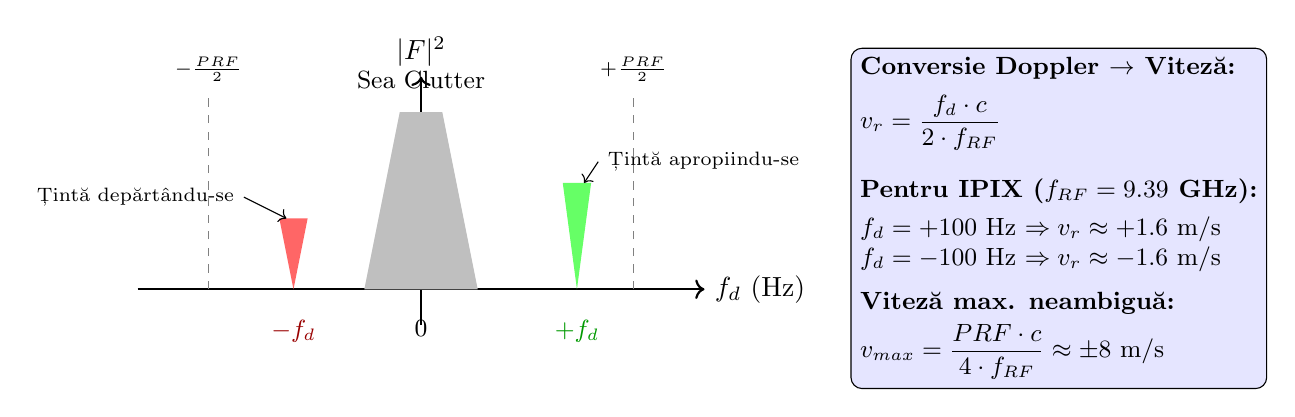
\begin{tikzpicture}[scale=0.9]

% Two-sided spectrum
\begin{scope}
    \draw[thick, ->] (-4,0) -- (4,0) node[right] {$f_d$ (Hz)};
    \draw[thick, ->] (0,-0.5) -- (0,3) node[above] {$|F|^2$};
    
    % Clutter at 0
    \fill[gray!50] (-0.8,0) -- (-0.3,2.5) -- (0.3,2.5) -- (0.8,0) -- cycle;
    \node[below] at (0,-0.3) {\small 0};
    
    % Target peak (positive Doppler)
    \fill[green!60] (2.2,0) -- (2.0,1.5) -- (2.4,1.5) -- cycle;
    \node[below, green!60!black] at (2.2,-0.3) {\small $+f_d$};
    
    % Target peak (negative Doppler)
    \fill[red!60] (-1.8,0) -- (-2.0,1.0) -- (-1.6,1.0) -- cycle;
    \node[below, red!60!black] at (-1.8,-0.3) {\small $-f_d$};
    
    % Labels
    \node[above] at (0,2.7) {\small Sea Clutter};
    \draw[->] (2.5,1.8) -- (2.3,1.5);
    \node[right, font=\scriptsize] at (2.5,1.8) {Țintă apropiindu-se};
    \draw[->] (-2.5,1.3) -- (-1.9,1.0);
    \node[left, font=\scriptsize] at (-2.5,1.3) {Țintă depărtându-se};
    
    % PRF limits
    \draw[dashed, gray] (-3,0) -- (-3,2.8);
    \draw[dashed, gray] (3,0) -- (3,2.8);
    \node[above, font=\scriptsize] at (-3,2.8) {$-\frac{PRF}{2}$};
    \node[above, font=\scriptsize] at (3,2.8) {$+\frac{PRF}{2}$};
\end{scope}

% Formulas
\begin{scope}[xshift=9cm, yshift=1cm]
    \node[draw, rounded corners, fill=blue!10, minimum width=5cm, align=left, font=\small] (formulas) {
        \textbf{Conversie Doppler $\rightarrow$ Viteză:}\\[0.5em]
        $v_r = \dfrac{f_d \cdot c}{2 \cdot f_{RF}}$\\[1em]
        \textbf{Pentru IPIX ($f_{RF} = 9.39$ GHz):}\\[0.3em]
        $f_d = +100$ Hz $\Rightarrow v_r \approx +1.6$ m/s\\
        $f_d = -100$ Hz $\Rightarrow v_r \approx -1.6$ m/s\\[0.5em]
        \textbf{Viteză max. neambiguă:}\\[0.3em]
        $v_{max} = \dfrac{PRF \cdot c}{4 \cdot f_{RF}} \approx \pm 8$ m/s
    };
\end{scope}

\end{tikzpicture}
\caption{Spectrul Doppler two-sided pentru date radar complexe I/Q. Frecvențele pozitive indică ținte care se apropie, cele negative ținte care se depărtează. Sea clutter-ul apare centrat la 0 Hz.}
\label{fig:doppler}
\end{figure}

%% =============================================================================
%% DIAGRAMA 6: Comparație parametri
%% =============================================================================
\section{Parametrii Implementării vs. Paper}

\begin{figure}[H]
\centering
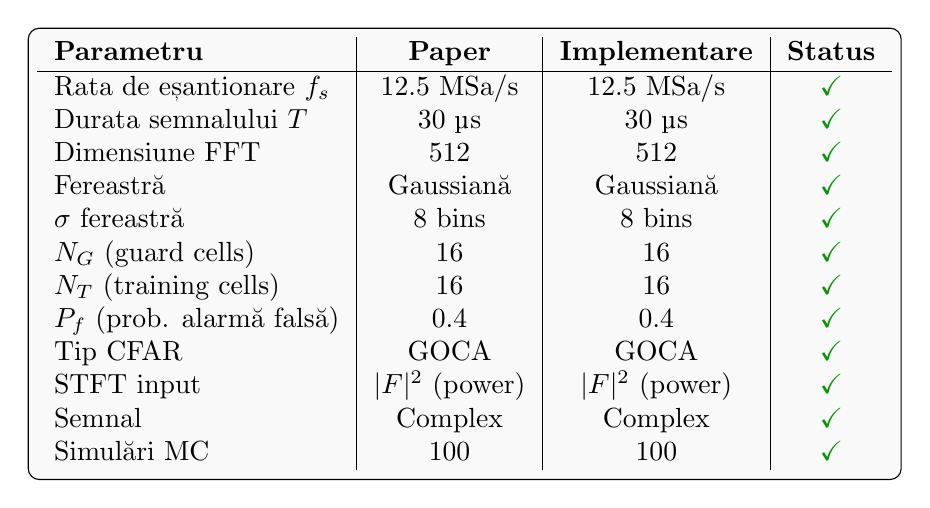
\begin{tikzpicture}
\node[draw, rounded corners, fill=gray!5] {
\begin{tabular}{l|c|c|c}
\textbf{Parametru} & \textbf{Paper} & \textbf{Implementare} & \textbf{Status} \\
\hline
Rata de eșantionare $f_s$ & 12.5 MSa/s & 12.5 MSa/s & \textcolor{green!60!black}{\checkmark} \\
Durata semnalului $T$ & 30 µs & 30 µs & \textcolor{green!60!black}{\checkmark} \\
Dimensiune FFT & 512 & 512 & \textcolor{green!60!black}{\checkmark} \\
Fereastră & Gaussiană & Gaussiană & \textcolor{green!60!black}{\checkmark} \\
$\sigma$ fereastră & 8 bins & 8 bins & \textcolor{green!60!black}{\checkmark} \\
$N_G$ (guard cells) & 16 & 16 & \textcolor{green!60!black}{\checkmark} \\
$N_T$ (training cells) & 16 & 16 & \textcolor{green!60!black}{\checkmark} \\
$P_f$ (prob. alarmă falsă) & 0.4 & 0.4 & \textcolor{green!60!black}{\checkmark} \\
Tip CFAR & GOCA & GOCA & \textcolor{green!60!black}{\checkmark} \\
STFT input & $|F|^2$ (power) & $|F|^2$ (power) & \textcolor{green!60!black}{\checkmark} \\
Semnal & Complex & Complex & \textcolor{green!60!black}{\checkmark} \\
Simulări MC & 100 & 100 & \textcolor{green!60!black}{\checkmark} \\
\end{tabular}
};
\end{tikzpicture}
\caption{Comparație între parametrii din paper (Abratkiewicz 2022) și implementarea curentă.}
\label{fig:params}
\end{figure}

%% =============================================================================
%% DIAGRAMA 7: Metrica RQF
%% =============================================================================
\section{Metrica de Evaluare: RQF}

\begin{figure}[H]
\centering
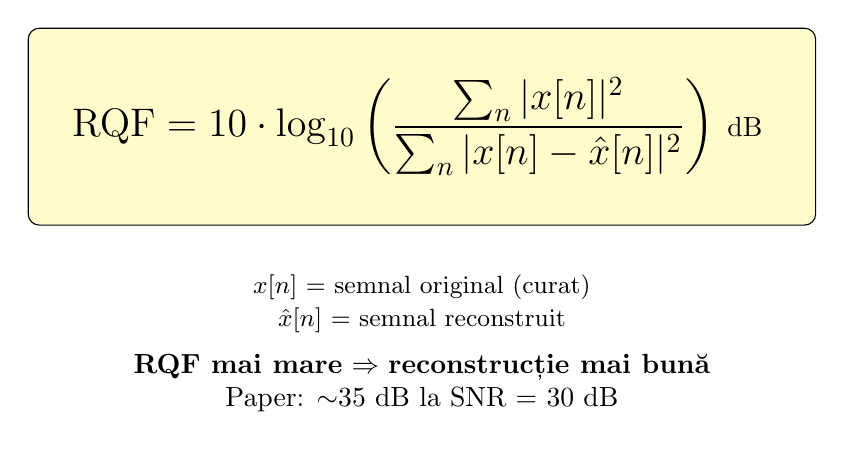
\begin{tikzpicture}
% RQF formula box
\node[draw, rounded corners, fill=yellow!20, minimum width=10cm, minimum height=2.5cm, align=center] (rqf) {
    \Large $\text{RQF} = 10 \cdot \log_{10} \left( \dfrac{\sum_n |x[n]|^2}{\sum_n |x[n] - \hat{x}[n]|^2} \right)$ \normalsize dB
};

\node[below=0.5cm of rqf, align=center] {
    \small $x[n]$ = semnal original (curat)\\
    \small $\hat{x}[n]$ = semnal reconstruit\\[0.5em]
    \textbf{RQF mai mare} $\Rightarrow$ \textbf{reconstrucție mai bună}\\
    Paper: $\sim$35 dB la SNR = 30 dB
};

\end{tikzpicture}
\caption{Formula RQF (Reconstruction Quality Factor) din Ecuația (15) a paper-ului.}
\label{fig:rqf}
\end{figure}

\end{document}
